\chapter*{Introduction}
\addcontentsline{toc}{chapter}{Introduction}

Since the cessation of full-scale nuclear testing, numerical simulation has become a central tool for the study and maintenance of nuclear deterrence capabilities. In this context, understanding high-energy-density physics phenomena is of major importance. These regimes involve extreme thermodynamic conditions, strong compressibility effects, shock waves, radiation transport, and hydrodynamic instabilities. Since such conditions cannot be fully reproduced using conventional laboratory experiments, dedicated experimental platforms and high-fidelity numerical simulations are required to investigate them.

Among these experimental platforms, Inertial Confinement Fusion (ICF) provides a privileged framework for studying matter under extreme pressure and temperature conditions. In ICF, a small capsule containing deuterium--tritium fuel is rapidly compressed by high-intensity laser beams. The ablation of the capsule outer layer generates an inward pressure, leading to the compression and heating of the fuel. If the implosion is sufficiently symmetric and efficient, thermonuclear reactions may occur before the target disassembles.

\begin{figure}[h]
\centering

\includegraphics[width=0.40\textwidth]{figures/intro/fci.png}
\caption{Schematic representation of an inertial confinement fusion target and laser-driven implosion process.}
\label{fig:icf_principle}
\end{figure}

A major difficulty in ICF lies in maintaining the stability of the implosion. Small perturbations initially present at material interfaces may grow during the acceleration phase and progressively degrade the compression quality. Among the hydrodynamic instabilities involved in this process, the Rayleigh--Taylor instability plays a central role. It occurs when a dense fluid is accelerated by a lighter one and leads to the development of characteristic bubble and spike structures. In the context of ICF, this instability may enhance turbulent mixing between the shell material and the fuel, thereby reducing the achievable temperature and compromising ignition conditions.

% \begin{figure}[h]
% \centering
% 
\includegraphics[width=0.75\textwidth]{figures/intro/rti_sketch.png}
% \caption{Illustration of the Rayleigh--Taylor instability developing at the interface between two fluids of different densities.}
% \label{fig:rti_scheme}
% \end{figure}

Predicting the evolution of the Rayleigh--Taylor instability remains challenging because of its non-linear, multi-scale, and eventually turbulent nature. Direct Numerical Simulations (DNS) provide a reference approach to study such flows, as they resolve the relevant spatial and temporal scales without relying on turbulence closure models. They therefore make it possible to generate accurate representations of the instability dynamics, from the early growth phase to more complex mixing regimes.

However, DNS are extremely expensive from a computational point of view. Their cost increases rapidly with the spatial resolution, the duration of the simulation, and the complexity of the physical model. As a consequence, only a limited number of simulations can generally be produced, which strongly constrains the size of the available datasets. This limitation is particularly important when considering data-driven approaches, whose performance often depends on the quantity and diversity of training data.

\begin{figure}[h]
\centering
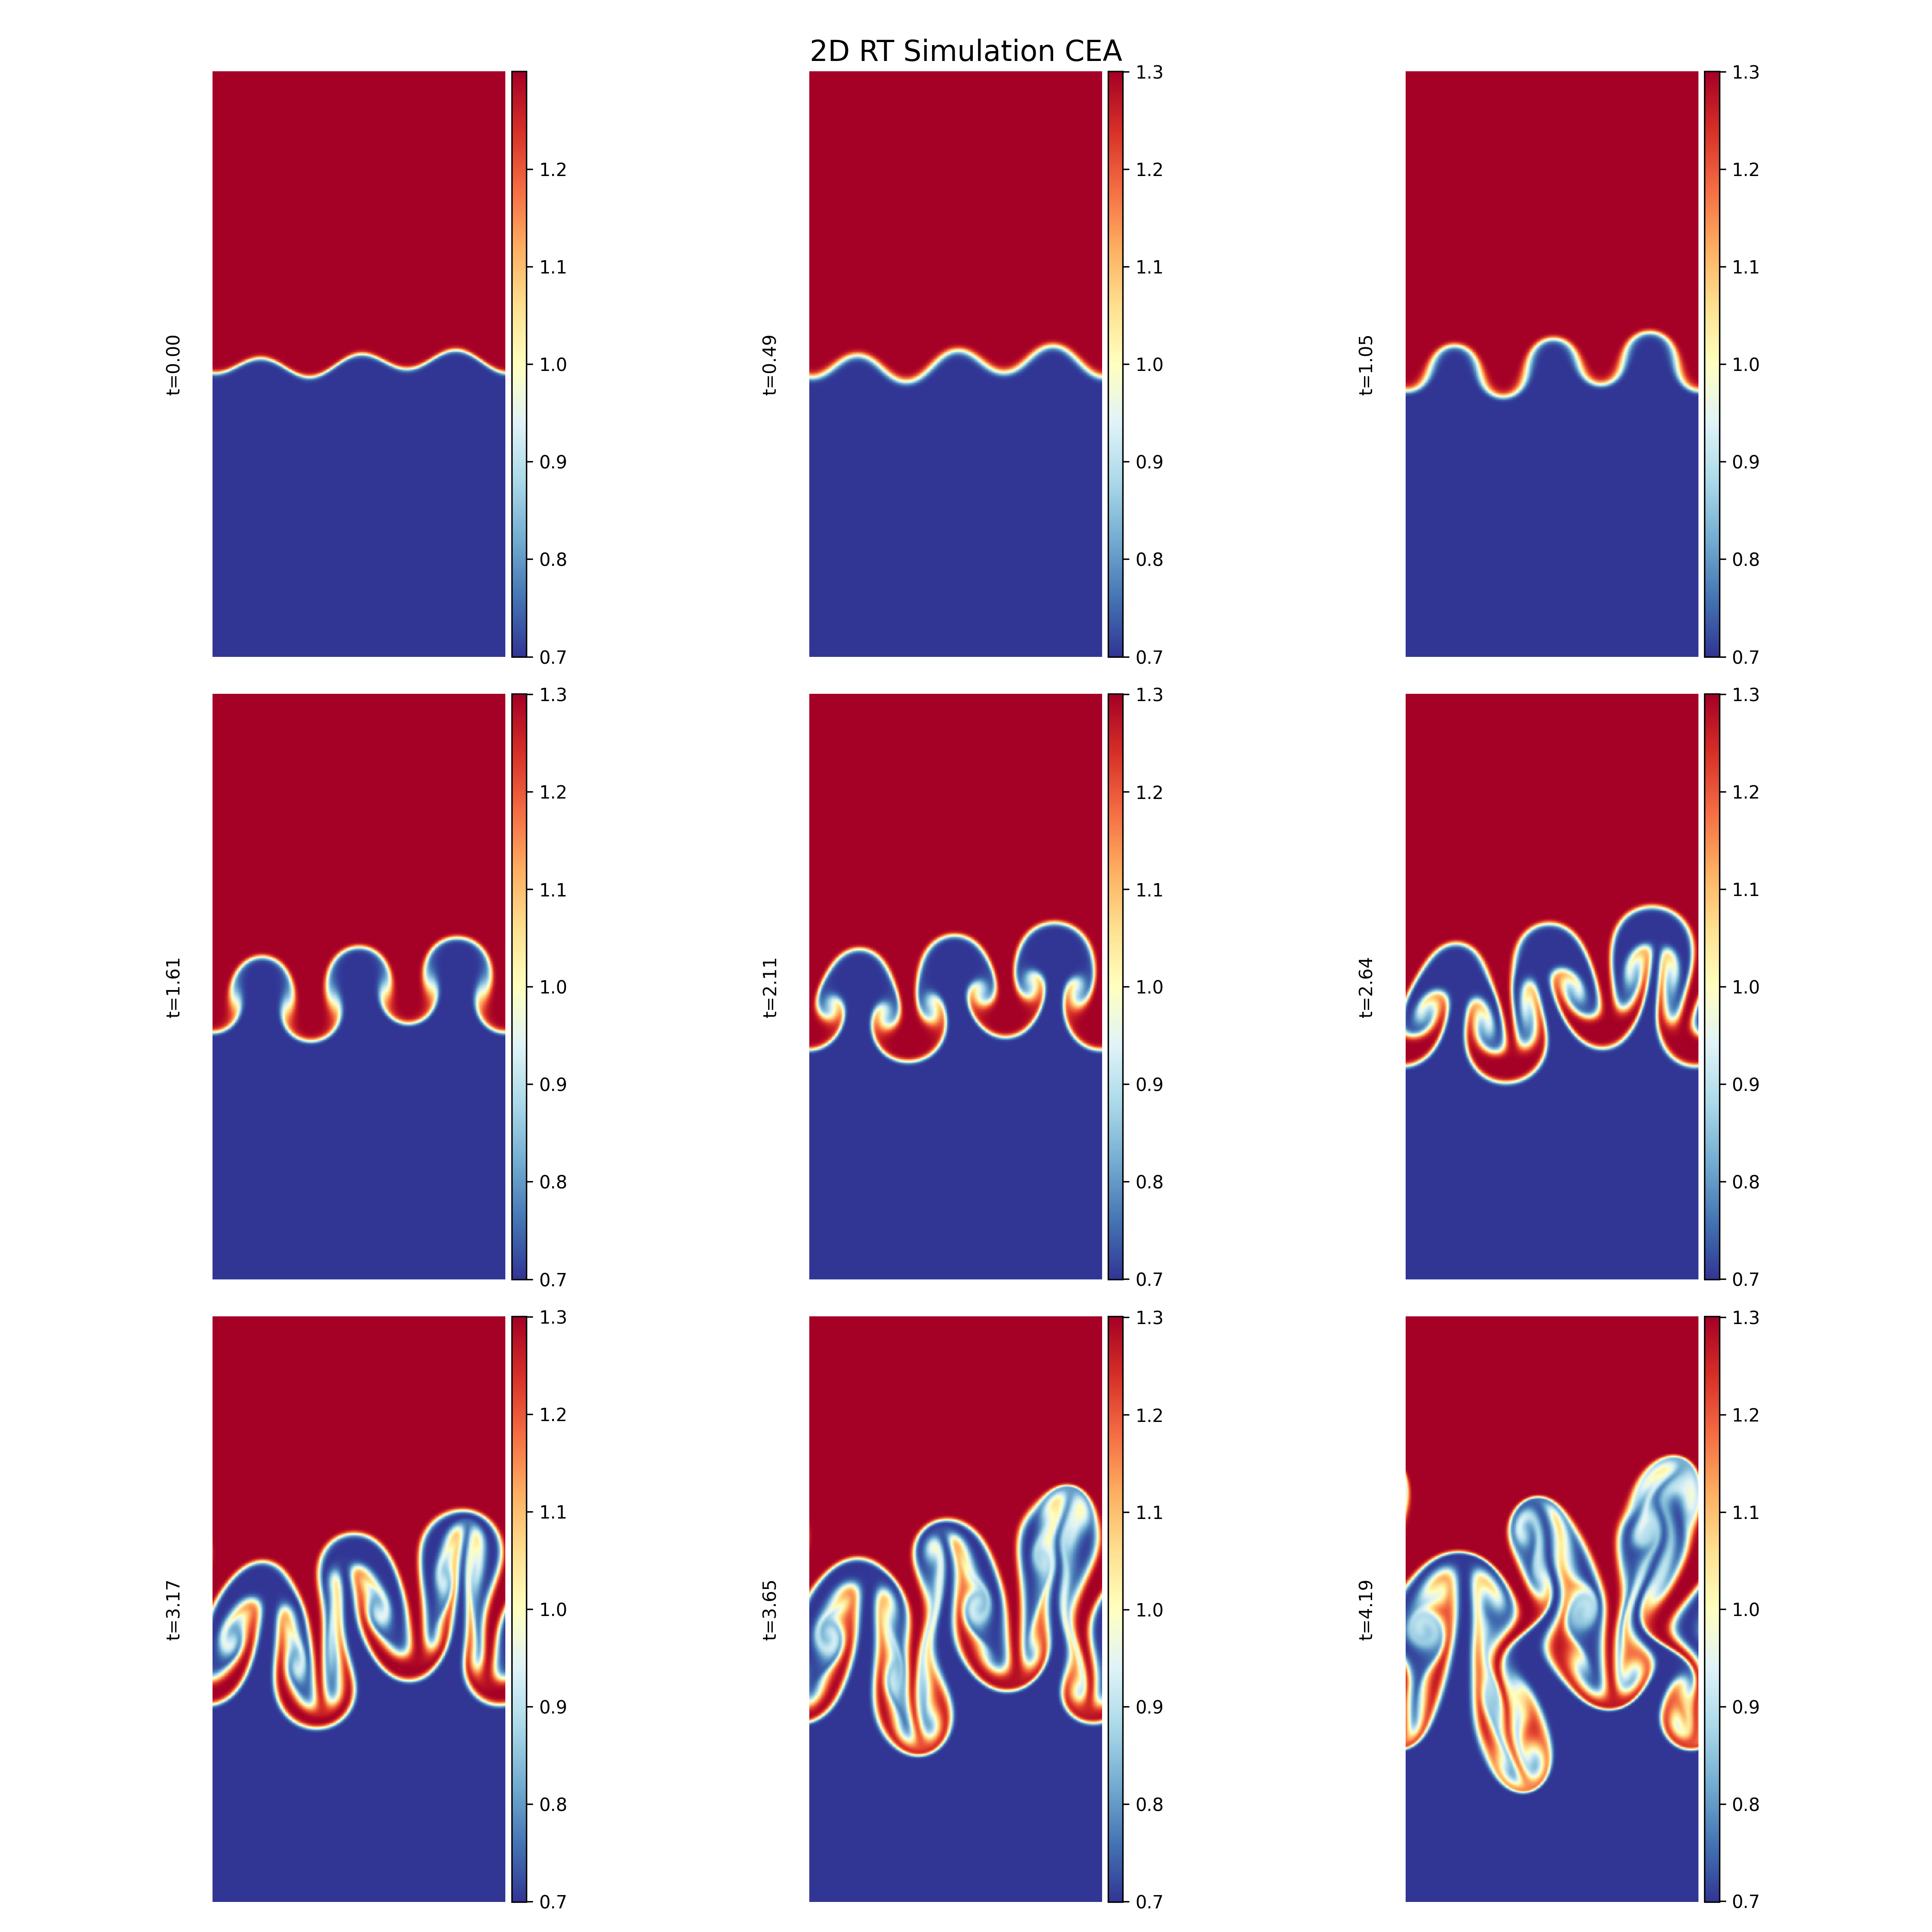
\includegraphics[width=0.8\textwidth]{figures/intro/RTCEA_simulation_2D.png}
\caption{Example of density field evolution obtained from Direct Numerical Simulations of the Rayleigh--Taylor instability}
\label{fig:dns_example}
\end{figure}

This context motivates the development of surrogate models able to reproduce, at a reduced computational cost, the statistical properties of fields generated by high-fidelity simulations. In recent years, machine learning methods have become increasingly attractive for this purpose, especially in computational fluid dynamics and plasma physics. Among them, diffusion models constitute a promising class of generative models, as they are designed to learn complex high-dimensional probability distributions.

The objective of this maseter thesis is to investigate the use of diffusion-based generative models for two-dimensional Rayleigh--Taylor instability fields obtained from DNS. More specifically, the goal is to approximate the probability distribution of the simulated density fields and to evaluate whether generated samples can reproduce the main visual and statistical features of the reference data. Because the available dataset is limited, particular attention is given to multi-scale representations. Wavelet decompositions are therefore considered as a possible way to exploit the hierarchical structure of the flow and improve the data efficiency of the generative model.

\begin{figure}[t]
\centering
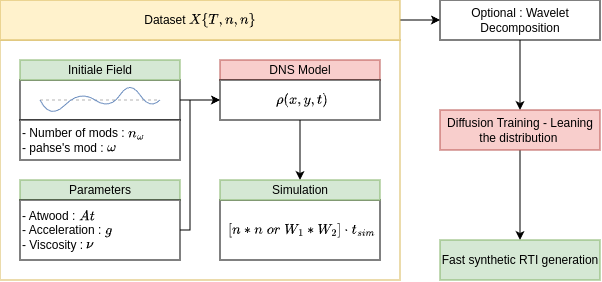
\includegraphics[width=0.8\textwidth]{figures/intro/pipeline_sktech.drawio.png}
\caption{General principle of the diffusion-based surrogate modeling approach used in this work}
\label{fig:diffusion_pipeline}
\end{figure}

The work presented in this report follows two main directions. First, a conventional diffusion model is implemented and trained directly on preprocessed Rayleigh--Taylor density fields, providing a baseline generative approach. Second, a wavelet-based diffusion strategy is investigated in order to assess whether a multi-resolution representation can improve the quality, stability, or data efficiency of the generation process. The comparison between these two approaches constitutes the central objective of this study.

% \section*{Manuscript Organization}

% This report is organized as follows.

% Chapter~1 introduces the physical and numerical framework of the Rayleigh--Taylor instability. It presents the main physical mechanisms involved in the instability, the DNS generation process, and the properties and limitations of the resulting dataset.

% Chapter~2 focuses on dimensionality reduction and multi-scale representations. Fourier-based methods, wavelet decompositions, and other reduction strategies are introduced and compared in the context of Rayleigh--Taylor density fields.

% Chapter~3 presents diffusion models and their adaptation to the considered dataset. It describes the baseline diffusion framework, the preprocessing pipeline, the model architecture, and the first generation results.

% Chapter~4 introduces the wavelet-based diffusion model. It details the proposed pipeline, presents the obtained results, and compares them with the baseline diffusion approach.
